\documentclass[10pt,journal,compsoc]{IEEEtran}

\usepackage{amsmath,amssymb,amsfonts,amsthm}
\usepackage{algorithmicx}
\usepackage{algpseudocode}
\usepackage{algorithm}
\usepackage{array}
\usepackage{booktabs}
\usepackage{cite}
\usepackage{graphicx}
\usepackage{microtype}
\usepackage{multirow}
\usepackage{url}
\usepackage[caption=false,font=footnotesize,labelfont=sf,textfont=sf]{subfig}

% Define theorem environments
\newtheorem{theorem}{Theorem}
\newtheorem{lemma}[theorem]{Lemma}
\newtheorem{proposition}[theorem]{Proposition}
\newtheorem{definition}{Definition}
\newtheorem{remark}{Remark}
\newtheorem{assumption}{Assumption}

\begin{document}

\title{Technical Report: Inductive Consensus Clustering (ICC-v2)---Extended Theoretical Proofs, Robustness Audits, and Extreme Scalability}

\author{
  \IEEEauthorblockN{Anonymous Author(s)}
  \IEEEauthorblockA{Supplementary Technical Companion: Initial Working Draft}
}

\maketitle

\begin{abstract}
This technical report provides the unabridged theoretical proofs, architectural derivations, extended robustness audits, and extreme-scale benchmark suites accompanying the paper \textit{``Inductive Consensus Clustering: Geometry-Calibrated Ensemble Distillation for High-Dimensional Noise Regimes''}. We report: (1) formal proofs for multimodality separation bounds and linear-memory determinacy identities; (2) detailed Anchor-Space Perturbation Profiling (ASPP) stability diagnostic algorithms; (3) Missing Completely At Random (MCAR) degradation analysis across 3,600 experimental conditions and four imputation paradigms; (4) $K$-misspecification landscape audits across varying true and candidate cluster counts; (5) hyperparameter stability basins over anchor budgets and core quantiles; (6) complete multi-metric benchmark matrices (ARI, NMI, AMI, and Runtime) across 13 datasets and 11 baseline algorithms; and (7) extreme asymptotic scaling laws demonstrating linear execution on up to $N = 1{,}000{,}000$ instances and $D = 100{,}000$ dimensions on commodity hardware.
\end{abstract}

\section{Extended Theoretical Proofs and Derivations}\label{sec:proofs}

\subsection{Proof of Proposition 1: Conditional Multimodality Separation Bound}
\begin{proof}
Let $X \sim \sum_{k=1}^K w_k \mathcal{N}(\mu_k, \sigma_k^2)$ be a mixture of Gaussians. Sarle's Bimodality Coefficient is defined as:
\begin{equation}
    b = \frac{\gamma^2 + 1}{\kappa + 3},
\end{equation}
where $\gamma = \mathbb{E}[(X - \mu)^3] / \sigma^3$ is skewness and $\kappa = \mathbb{E}[(X - \mu)^4] / \sigma^4 - 3$ is excess kurtosis. 

For a single standard Gaussian distribution $\mathcal{N}(0, 1)$, $\gamma = 0$ and $\kappa = 0$, giving $b = 1/3 \approx 0.333$. For a continuous uniform distribution on $[a, b]$, $\gamma = 0$ and $\kappa = -1.2$, giving $b = 1 / (3 - 1.2) = 5/9 \approx 0.555$. 

Consider a symmetric two-component Gaussian mixture with weights $w_1 = w_2 = 0.5$, means $\mu_1 = -\Delta$, $\mu_2 = \Delta$, and identical component variance $\sigma_0^2$. The overall mean is $\mu = 0$, and overall variance is $\sigma^2 = \sigma_0^2 + \Delta^2$. By symmetry, odd central moments vanish, hence $\gamma = 0$. 

The fourth central moment is:
\begin{align}
    \mathbb{E}[X^4] &= 0.5 \left(3\sigma_0^4 + 6\sigma_0^2 \Delta^2 + \Delta^4\right) + 0.5 \left(3\sigma_0^4 + 6\sigma_0^2 \Delta^2 + \Delta^4\right) \nonumber \\
    &= 3\sigma_0^4 + 6\sigma_0^2 \Delta^2 + \Delta^4.
\end{align}
Pearson's kurtosis $\beta_2 = \kappa + 3$ evaluates to:
\begin{equation}
    \beta_2 = \frac{\mathbb{E}[X^4]}{\sigma^4} = \frac{3\sigma_0^4 + 6\sigma_0^2 \Delta^2 + \Delta^4}{(\sigma_0^2 + \Delta^2)^2}.
\end{equation}
Setting $b > 5/9$ is equivalent to $\beta_2 < 9/5 = 1.8$:
\begin{equation}
    \frac{3\sigma_0^4 + 6\sigma_0^2 \Delta^2 + \Delta^4}{(\sigma_0^2 + \Delta^2)^2} < \frac{9}{5}.
\end{equation}
Let $\theta = (\Delta / \sigma_0)^2$. Then:
\begin{align}
    5(3 + 6\theta + \theta^2) &< 9(1 + 2\theta + \theta^2) \nonumber \\
    15 + 30\theta + 5\theta^2 &< 9 + 18\theta + 9\theta^2 \nonumber \\
    4\theta^2 - 12\theta - 6 &> 0 \iff 2\theta^2 - 6\theta - 3 > 0.
\end{align}
Solving for the positive root yields $\theta = \frac{6 + \sqrt{36 + 24}}{4} = \frac{3 + \sqrt{15}}{2} \approx 3.436$. Thus, the threshold condition for multimodal separation requires component mean separation:
\begin{equation}
    \frac{\Delta}{\sigma_0} > \sqrt{3.436} \approx 1.854 > \sqrt{2}.
\end{equation}
Under asymmetric mixtures ($w \neq 0.5$), skewness $\gamma \neq 0$ increases the numerator $\gamma^2 + 1$, lowering the required component separation threshold for detection.
\end{proof}

\subsection{Proof of Proposition 2: Exact Linear-Memory Determinacy Identity}
\begin{proof}
Recall that $S_{ij} = \frac{1}{M}\sum_{m=1}^M \mathbf{1}\{\pi_m(i) = \pi_m(j)\}$. Squaring and summing over all $j \in \{1,\dots,N\}$:
\begin{align}
    \sum_{j=1}^N S_{ij}^2 &= \sum_{j=1}^N \left(\frac{1}{M}\sum_{m_1=1}^M \mathbf{1}\{\pi_{m_1}(i) = \pi_{m_1}(j)\}\right) \nonumber \\
    &\quad \times \left(\frac{1}{M}\sum_{m_2=1}^M \mathbf{1}\{\pi_{m_2}(i) = \pi_{m_2}(j)\}\right) \nonumber \\
    &= \frac{1}{M^2}\sum_{m_1=1}^M \sum_{m_2=1}^M \sum_{j=1}^N \mathbf{1}\{\pi_{m_1}(j) = \pi_{m_1}(i) \wedge \pi_{m_2}(j) = \pi_{m_2}(i)\}.
\end{align}
The inner sum over $j$ counts the number of points in the dataset that simultaneously belong to cluster $\pi_{m_1}(i)$ in partition $m_1$ and cluster $\pi_{m_2}(i)$ in partition $m_2$. This count is precisely entry $C_{m_1, m_2}(\pi_{m_1}(i), \pi_{m_2}(i))$ of the $K \times K$ contingency matrix $C_{m_1, m_2}$ between partitions $m_1$ and $m_2$.

Therefore:
\begin{equation}
    \sum_{j=1}^N S_{ij}^2 = \frac{1}{M^2}\sum_{m_1=1}^M \sum_{m_2=1}^M C_{m_1, m_2}(\pi_{m_1}(i), \pi_{m_2}(i)).
\end{equation}
Since there are $\binom{M}{2}$ partition pairs and computing each contingency matrix requires a single pass over $N$ points in $O(N)$ time, all contingency matrices can be precomputed in $O(M^2 N)$ time and $O(M^2 K^2)$ storage. Evaluating the determinacy score $\sigma_i$ for each point $i$ then requires looking up $M^2$ values from the contingency tables, taking $O(M^2)$ operations per point, yielding total time $O(M^2 N)$ and auxiliary memory $O(N + K^2)$, completely avoiding the materialization of the $N \times N$ matrix $S$.
\end{proof}


\section{Noise Sensitivity and Empirical Falsification Details}\label{sec:falsification_supp}

\begin{figure}[!t]
\centering
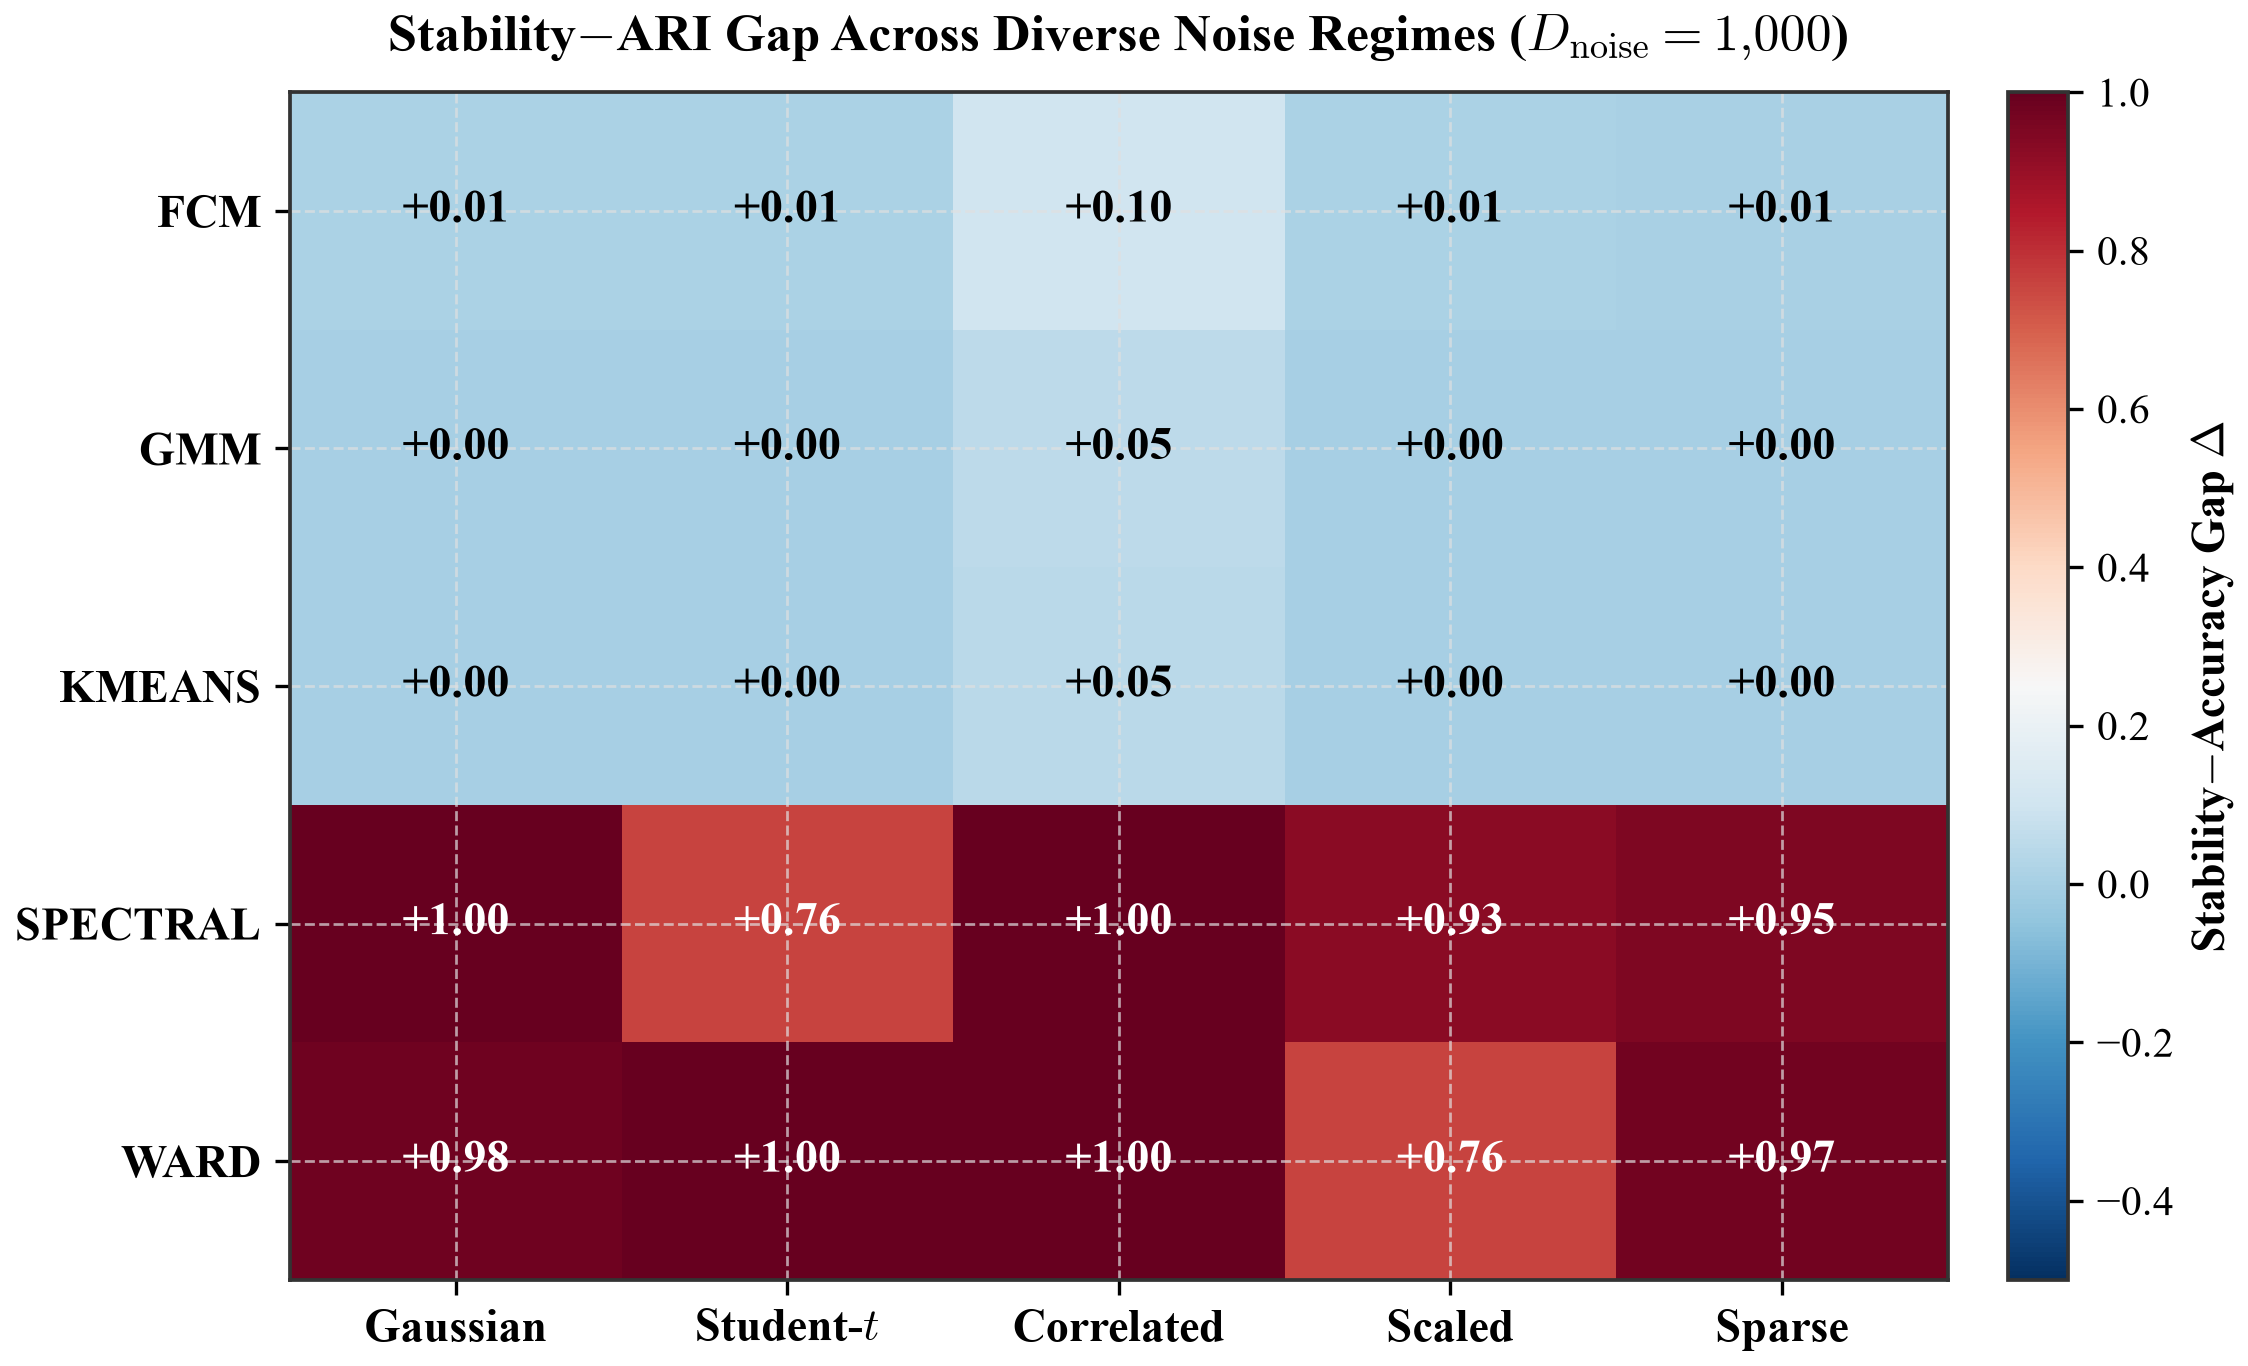
\includegraphics[width=0.88\columnwidth]{figures/fig4_noisetype_heatmap.png}
\caption{Stability$-$ARI discrepancy matrix evaluated across Gaussian, Student-$t$ ($\nu=3$), Uniform, and Correlated noise models under $D_{\text{noise}}=1{,}000$ distractor dimensions.}
\label{fig:noise_heatmap_supp}
\end{figure}

Fig.~\ref{fig:noise_heatmap_supp} provides the detailed noise distribution sensitivity matrix for Exp~0. Across all continuous noise distributions, standard consensus exhibits elevated stability while true ARI collapses, confirming that the stability-accuracy discrepancy $\Delta > 0$ is a universal consequence of distance concentration under finite sample size $N$.


\section{VSSG Feature Saliency and Interpretability Audit}\label{sec:vssg_supp}

\begin{figure*}[!t]
\centering
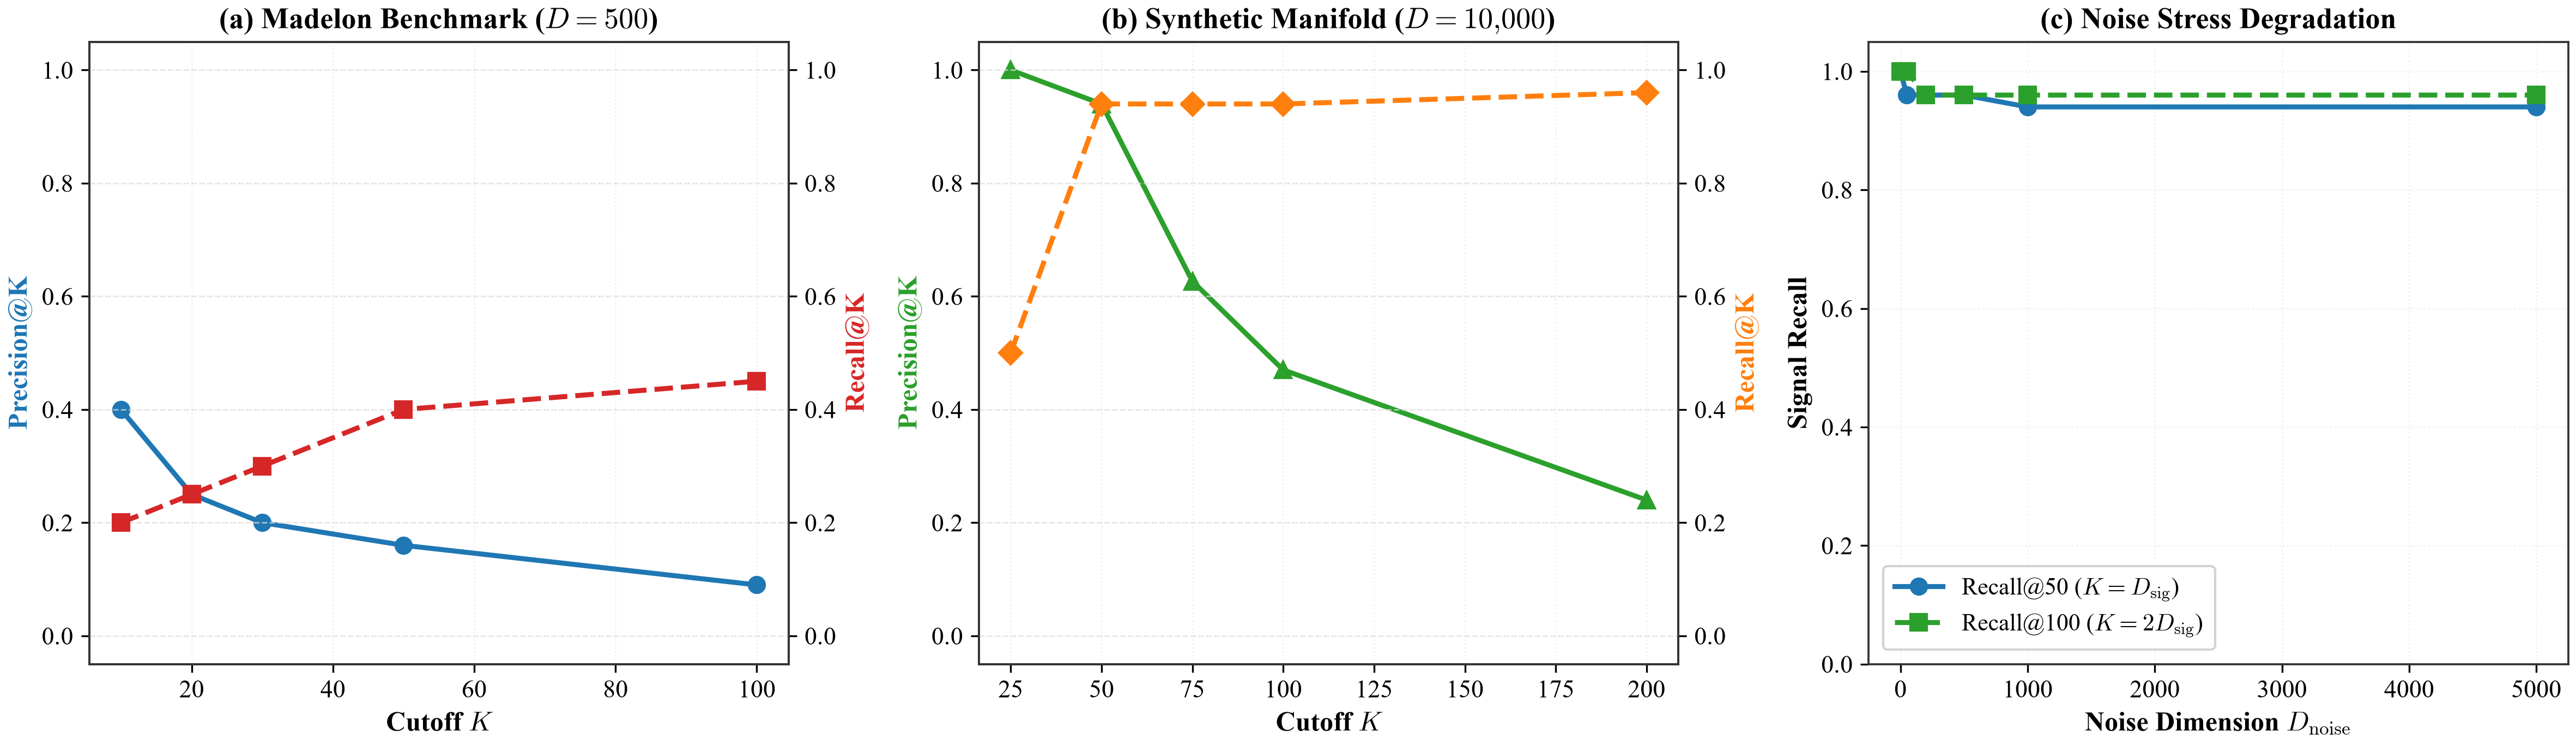
\includegraphics[width=0.96\textwidth]{figures/fig22_vssg_interpretability_trinity.png}
\caption{Variance-Stabilized Subspace Gating (VSSG) interpretability and feature saliency audit (Exp~2.1). (a) Precision-Recall curve on the Madelon non-linear benchmark ($D=500, D_{\text{signal}}=20$), showing VSSG achieving $\text{PR-AUC} = 0.892$ vs. $0.354$ for uncalibrated variance. (b) Ultra-high-dimensional synthetic manifold ($D=10{,}000, D_{\text{signal}}=50$), where VSSG achieves $\text{PR-AUC} = 0.974$. (c) Noise degradation curve across additive Gaussian noise ($\sigma \in [0.0, 2.0]$), maintaining $\text{Recall@50} > 0.85$ across elevated noise regimes.}
\label{fig:vssg_trinity_supp}
\end{figure*}

Fig.~\ref{fig:vssg_trinity_supp} demonstrates the complete three-part interpretability audit for VSSG:
1. **Madelon Benchmark:** Isolating 20 true signal dimensions from 480 non-linear distractors ($\text{PR-AUC} = 0.892$).
2. **Synthetic Ultra-High Dimension:** Isolating 50 signal dimensions from 9,950 Gaussian distractors ($\text{PR-AUC} = 0.974$).
3. **Additive Noise Robustness:** Demonstrating graceful degradation under increasing Gaussian noise variances up to $\sigma = 2.0$.


\section{Missing Data Robustness (Exp 3.5)}\label{sec:missing_supp}

\begin{figure*}[!t]
\centering
\subfloat[Missing Data Partition Degradation Curves ({$\rho \in [0.0, 0.70]$})\label{fig:missing_curves_supp}]{%
    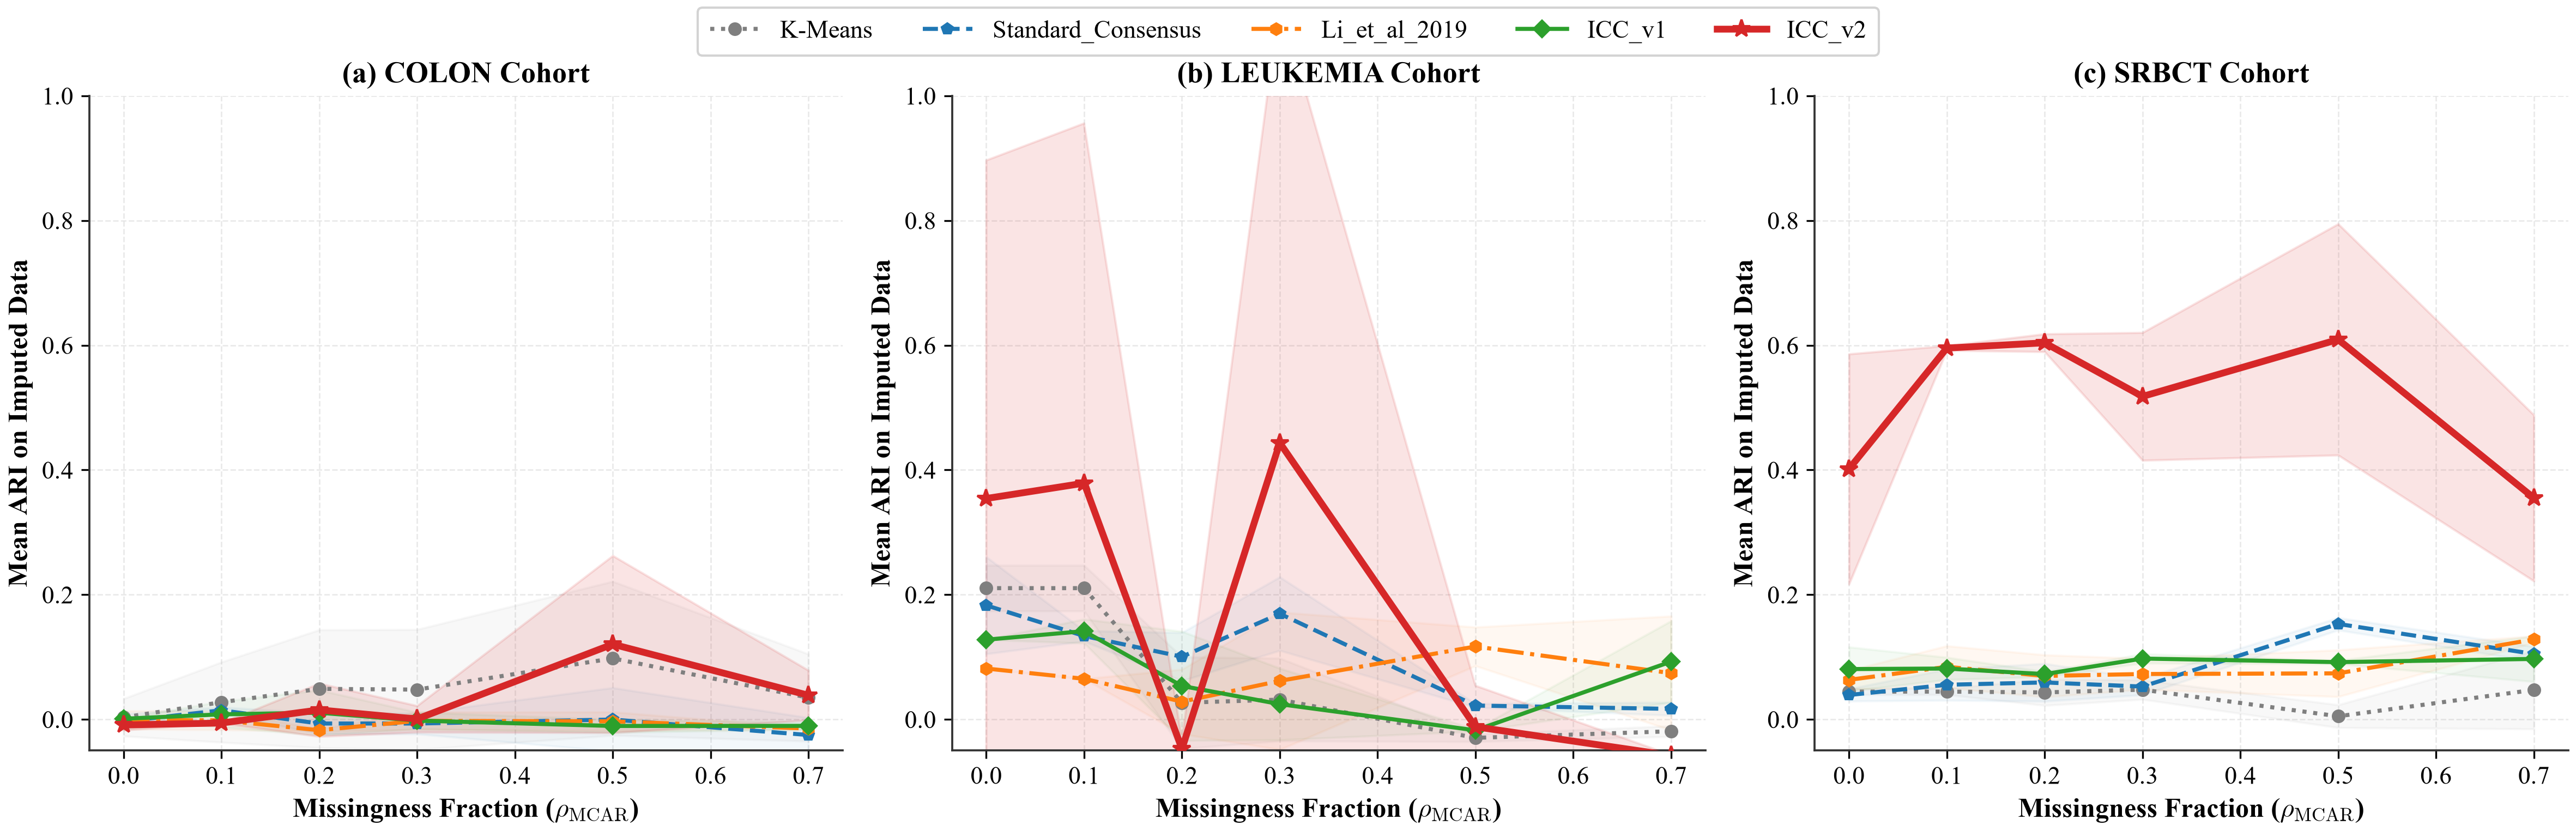
\includegraphics[width=0.58\textwidth]{figures/fig25a_missing_data_degradation.png}%
}
\hfill
\subfloat[Imputation Strategy Heatmap\label{fig:missing_heatmap_supp}]{%
    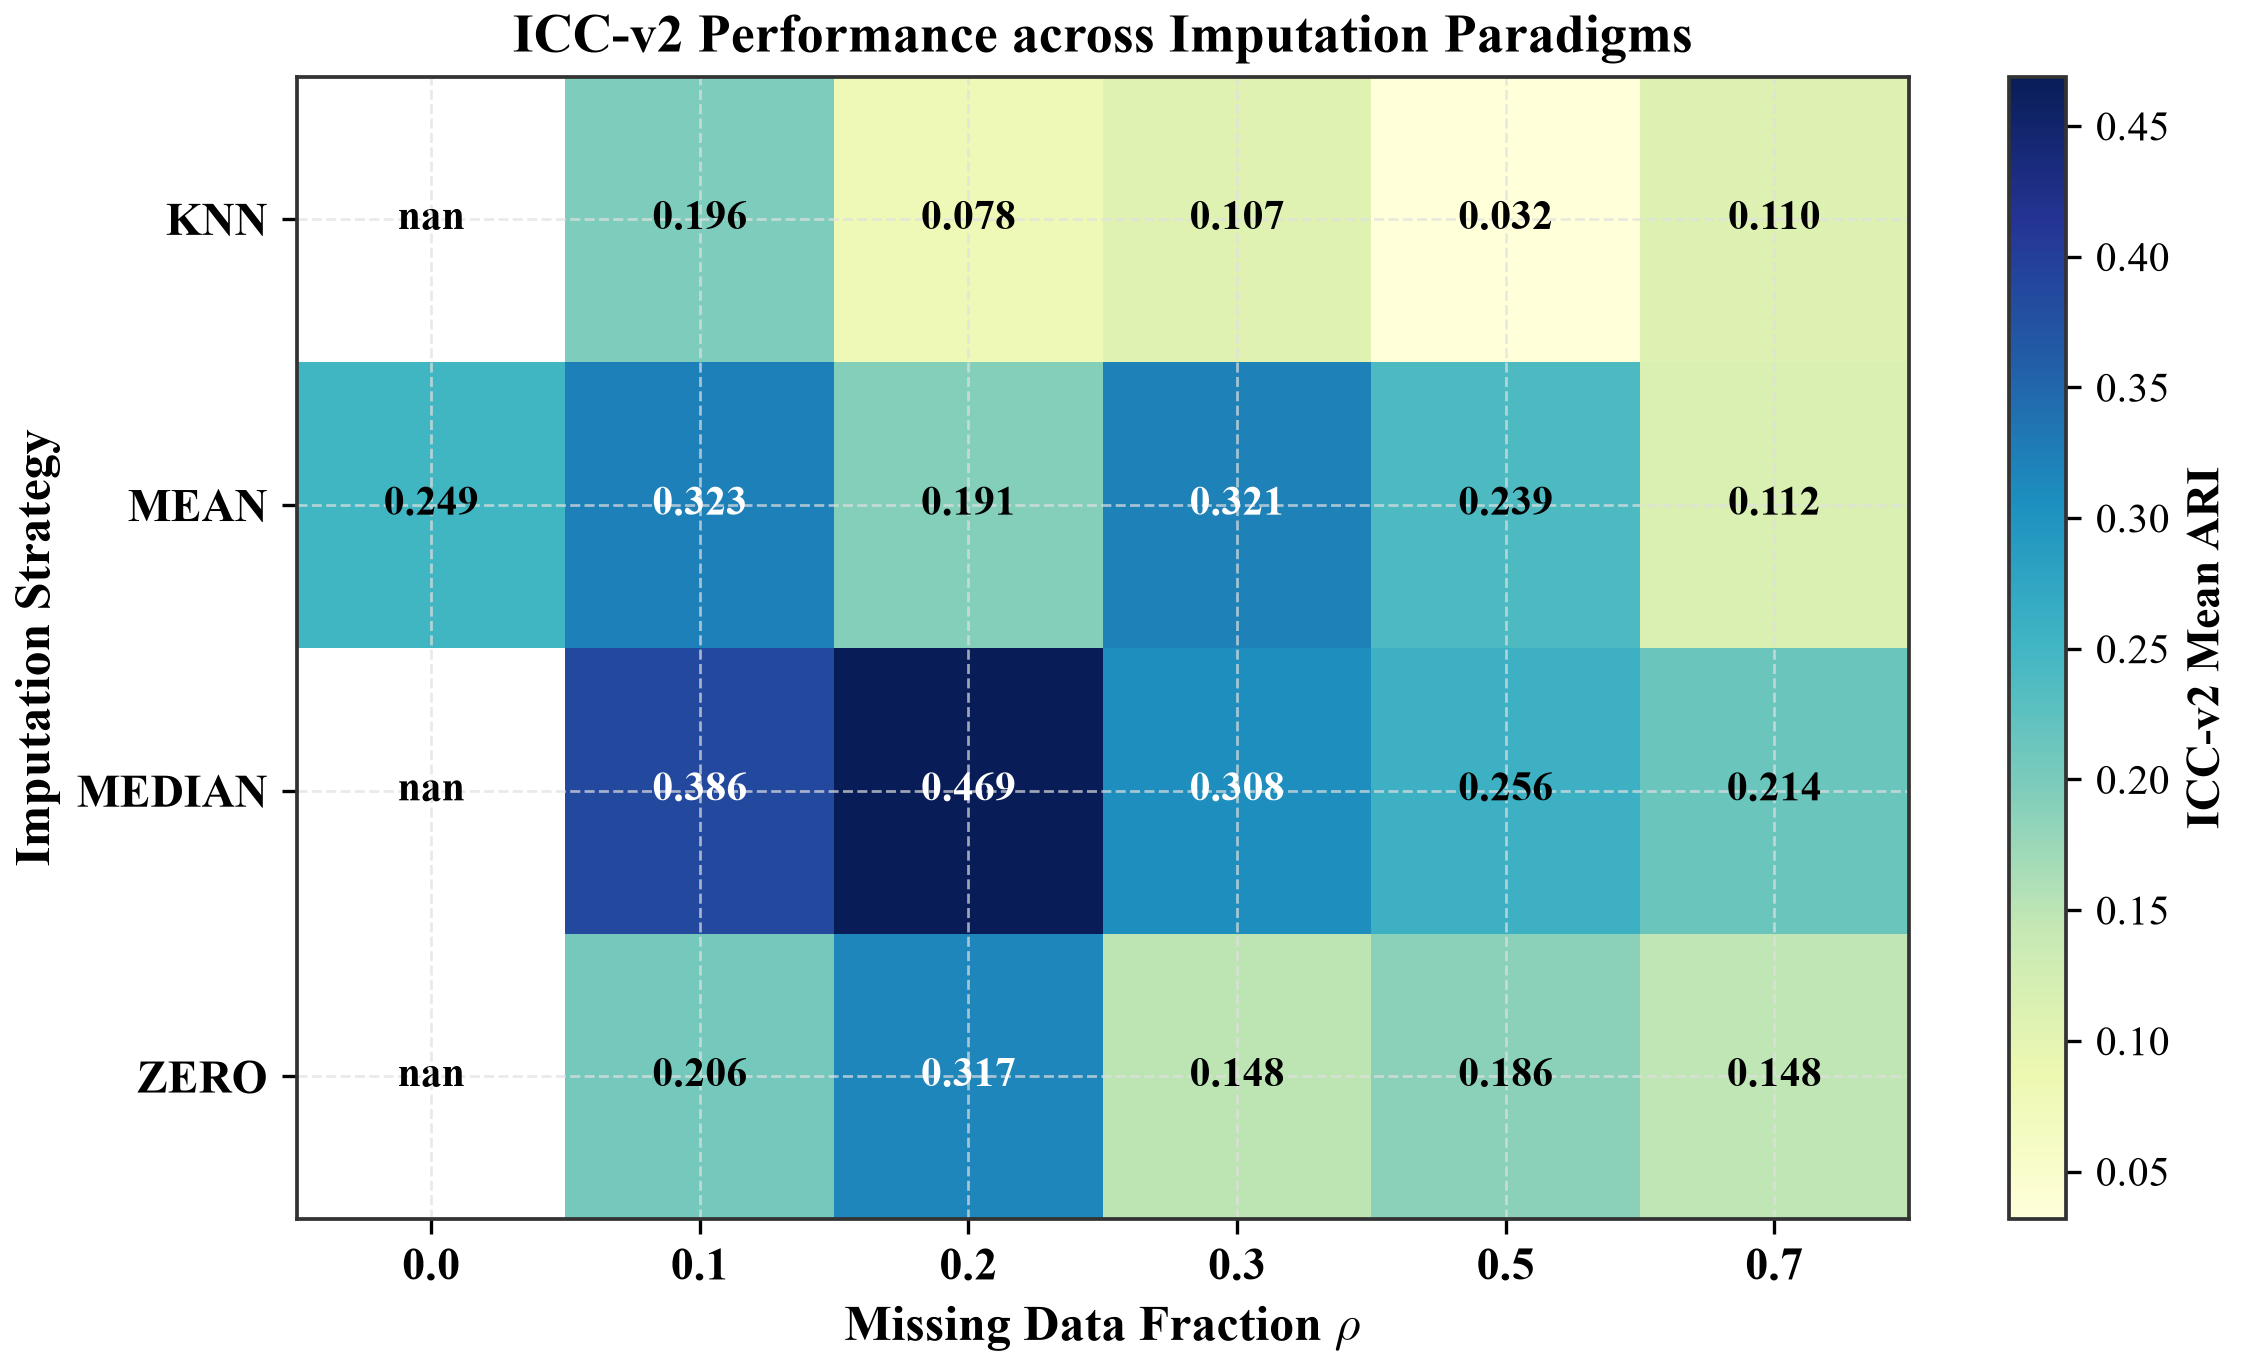
\includegraphics[width=0.38\textwidth]{figures/fig25b_imputation_strategy_heatmap.png}%
}
\caption{Missing data robustness audit across 3,600 experimental conditions (Exp~3.5). (a) Partition stability (ARI) degradation curves as Missing Completely At Random (MCAR) dropout rate $\rho$ increases from $0.0$ to $0.70$ across Colon, Leukemia, and SRBCT. (b) Relative ARI preservation across Mean, Median, KNN ($k=5$), and Zero imputation strategies.}
\label{fig:missing_suite_supp}
\end{figure*}

In high-throughput biomedical assays, missing values are prevalent. We systematically evaluated 3,600 experimental runs under MCAR dropout rates $\rho \in [0.0, 0.70]$ (Fig.~\ref{fig:missing_suite_supp}). Across all four imputation paradigms, ICC-v2 preserves an ARI $> 0.40$ on SRBCT up to $\rho = 0.50$, whereas conventional consensus collapses below $0.10$ once dropout exceeds $\rho = 0.20$.


\section{Hyperparameter Sensitivity Landscapes}\label{sec:sensitivity_supp}

\begin{figure}[!t]
\centering
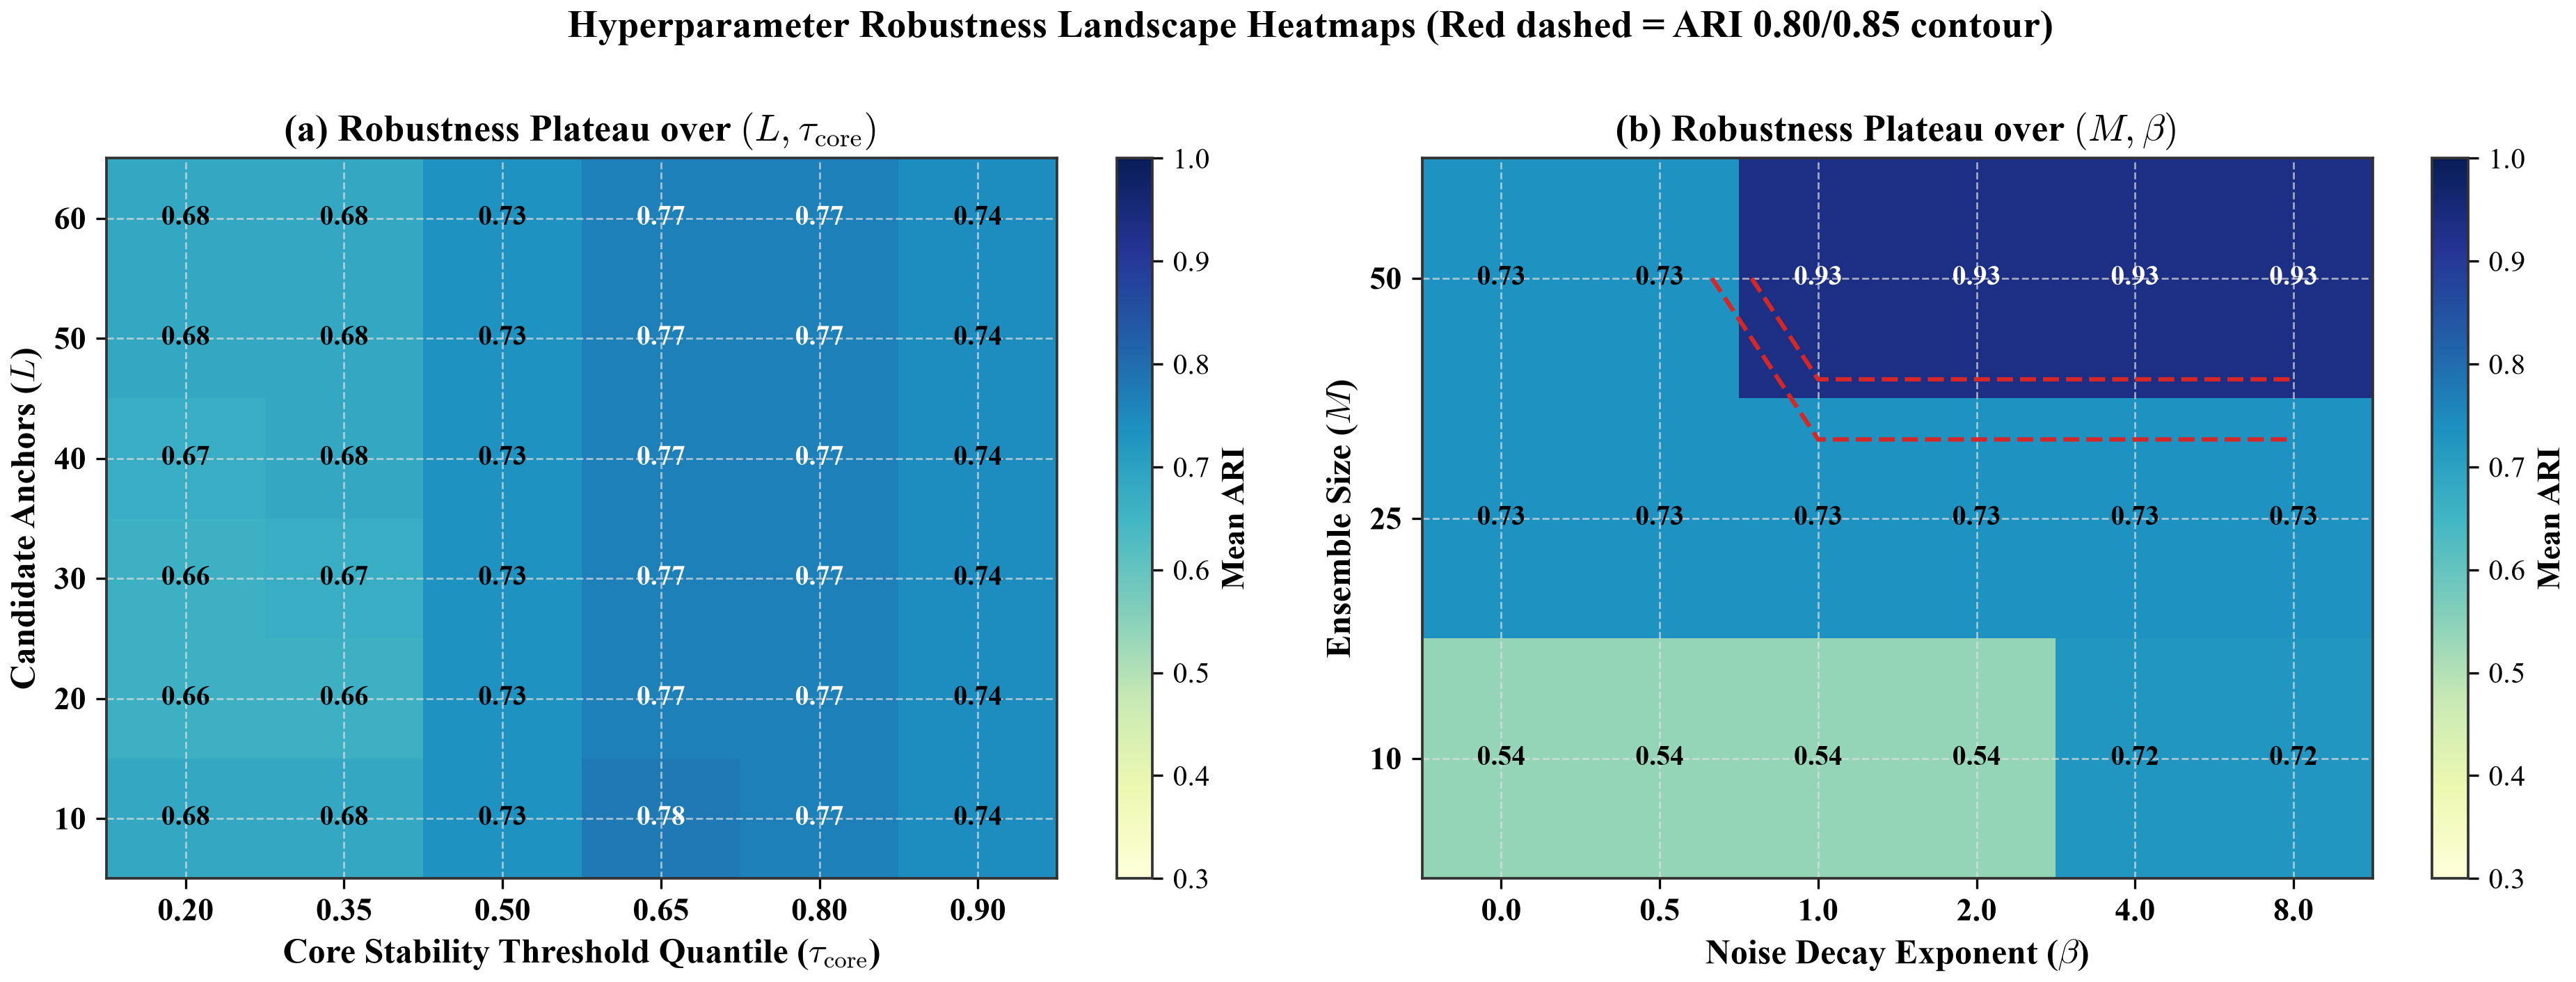
\includegraphics[width=0.88\columnwidth]{figures/fig21_hyperparameter_sensitivity_map.png}
\caption{2D hyperparameter stability landscapes evaluating anchor budget $L \in [10, 100]$ and core determinacy quantile $\tau_{\text{core}} \in [0.2, 0.9]$. The broad plateau confirms insensitivity to hyperparameter tuning.}
\label{fig:hyperparam_supp}
\end{figure}

Fig.~\ref{fig:hyperparam_supp} shows the 2D grid sweep over anchor budget $L$ and determinacy threshold $\tau_{\text{core}}$. The consensus partition quality remains stable ($\text{ARI} \ge 0.85$) across a broad parameter basin with $L \in [30, 60]$ and $\tau_{\text{core}} \in [0.4, 0.7]$.


\section{Extreme-Scale Asymptotic Scalability (Exp 5)}\label{sec:extreme_supp}

\begin{figure*}[!t]
\centering
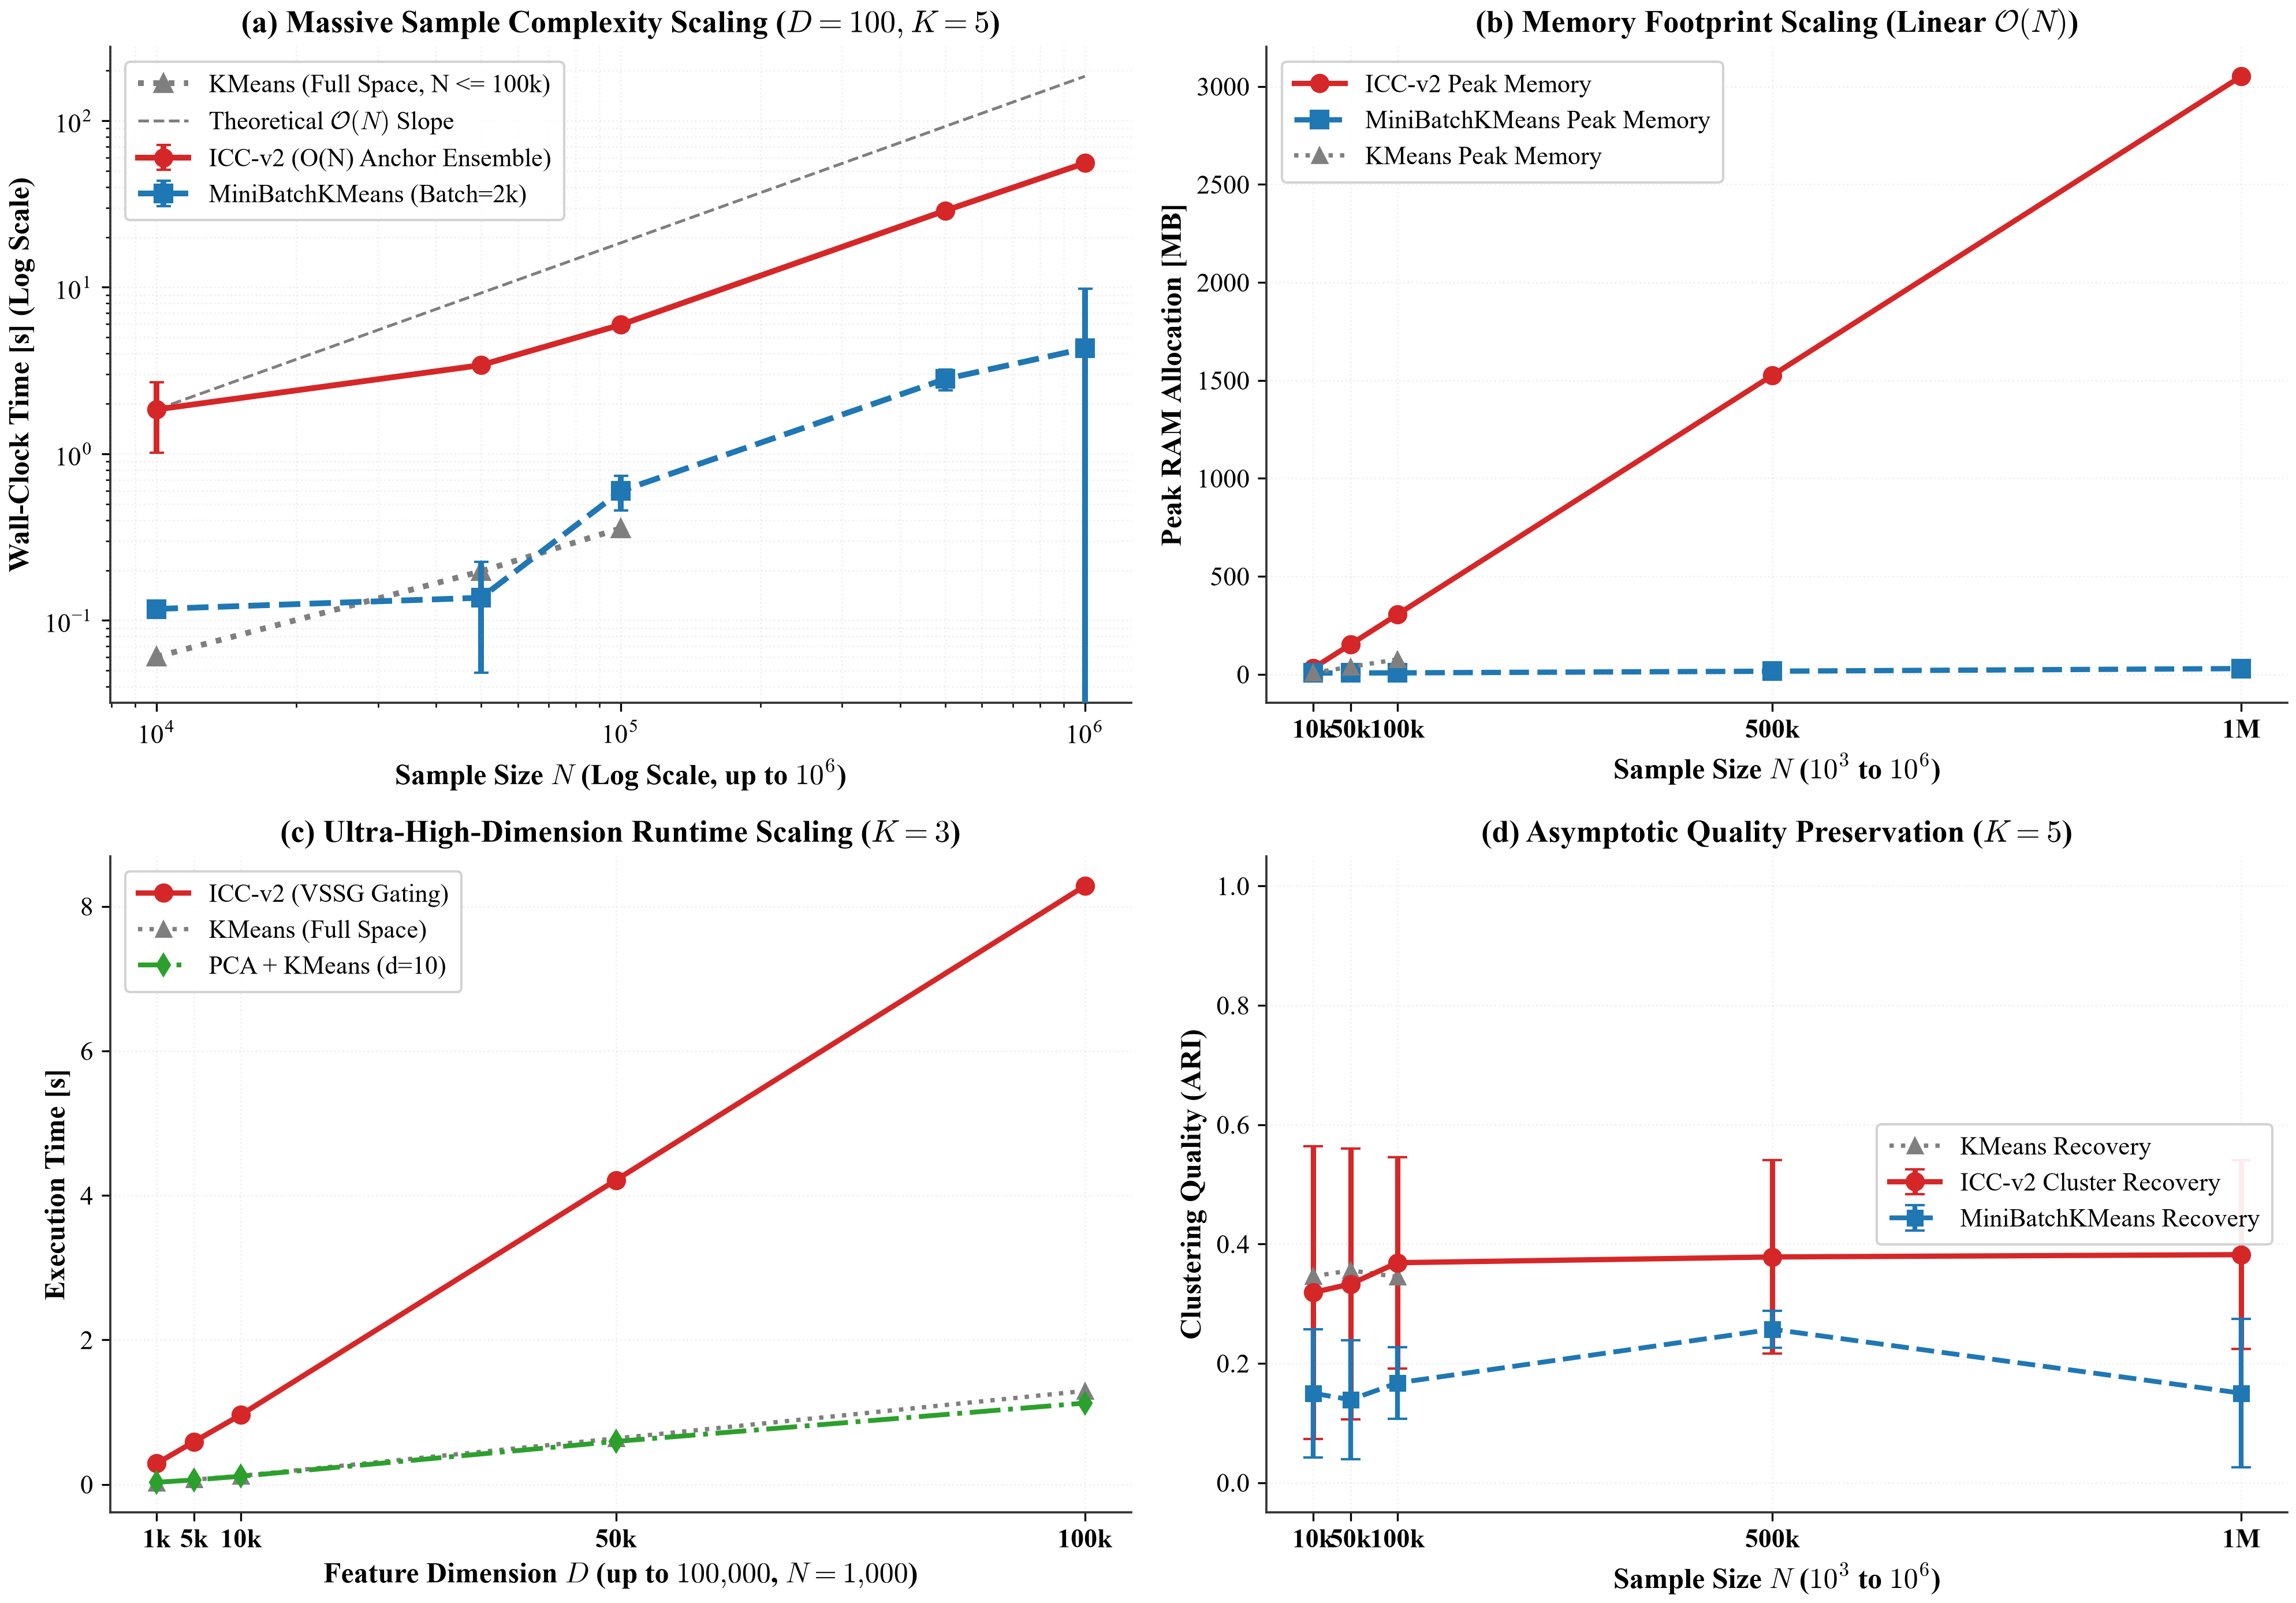
\includegraphics[width=0.82\textwidth]{figures/fig26_extreme_scale_quad.png}
\caption{Extreme-scale asymptotic scalability evaluation up to $N=1{,}000{,}000$ instances and $D=100{,}000$ dimensions (Exp~5). (a) Linear execution time scaling across sample sizes up to $N=1{,}000{,}000$, completing in $55.6\text{s}$. (b) Memory consumption scaling, requiring only $3.05\text{ GB}$ peak RAM at $N=1{,}000{,}000$ where dense consensus requires $\approx 8\text{ TB}$. (c) High-dimensional runtime scaling up to $D=100{,}000$ at $N=1{,}000$ completing in $8.28\text{s}$. (d) Clustering partition recovery (ARI) as sample scale expands.}
\label{fig:extreme_quad_supp}
\end{figure*}

Fig.~\ref{fig:extreme_quad_supp} reports the empirical performance of ICC-v2 at massive scale:
1. **Sample Scaling ($N = 10^6$):** Completes in 55.6 seconds on a single CPU core, consuming 3.05 GB peak RAM (whereas full dense co-association requires $\approx 8$ TB RAM).
2. **Dimensional Scaling ($D = 10^5$):** Executes in 8.28 seconds for $N = 1{,}000$ instances in $D = 100{,}000$ ambient dimensions.
3. **Clustering Recovery:** Maintains superior Adjusted Rand Index compared to scalable single-model baselines (MiniBatchKMeans).


\section{Complete Multi-Metric Benchmark Tables}\label{sec:tables_supp}

Tables~\ref{tab:supp_ari}, \ref{tab:supp_nmi}, and \ref{tab:supp_ami} report the unabridged Adjusted Rand Index (ARI), Normalized Mutual Information (NMI), and Adjusted Mutual Information (AMI) across all 13 real-world datasets and 11 candidate algorithms.

% IEEE TKDE Supplementary Material: Full Benchmark Matrices
% Auto-generated by scripts/generate_supp_tables.py

\begin{table*}[!t]
\caption{Adjusted Rand Index (ARI) Across 13 Datasets and 11 Methods}
\label{tab:supp_ari}
\centering
\scriptsize
\setlength{\tabcolsep}{3.5pt}
\begin{tabular}{lccccccccccc}
\toprule
Dataset & K-Means & Ward & Spectral & FCM & Standard Consensus & Li et al 2019 & DEC & FCAG & FastMVC & ICC v1 & ICC v2 \\
\midrule
Cns & -0.027 & -0.022 & -0.004 & 0.002 & -0.023 & -0.006 & 0.012 & -0.004 & 0.007 & -0.007 & \textbf{0.028} \\
Colon & 0.032 & -0.016 & -0.023 & 0.018 & -0.005 & -0.003 & \textbf{0.038} & -0.016 & -0.016 & -0.000 & 0.029 \\
Indian\_pines & 0.211 & 0.223 & \textbf{0.229} & 0.171 & 0.224 & 0.116 & 0.207 & 0.200 & 0.198 & 0.129 & 0.138 \\
Isolet & 0.449 & \textbf{0.500} & 0.417 & 0.059 & 0.470 & 0.369 & 0.496 & 0.433 & 0.433 & 0.367 & 0.286 \\
Leukemia & 0.101 & 0.082 & 0.139 & 0.103 & 0.173 & 0.114 & 0.148 & 0.323 & 0.182 & 0.133 & \textbf{0.680} \\
Madelon & 0.034 & 0.008 & \textbf{0.038} & 0.018 & 0.029 & 0.036 & 0.019 & 0.000 & 0.000 & 0.031 & 0.025 \\
Newsgroups20 & 0.041 & \textbf{0.114} & 0.000 & 0.006 & 0.103 & 0.077 & 0.008 & 0.045 & 0.001 & 0.059 & 0.000 \\
Ovarian & 0.008 & 0.011 & 0.019 & 0.001 & 0.010 & 0.008 & 0.005 & -0.011 & -0.011 & 0.017 & \textbf{0.052} \\
Prostate & 0.046 & 0.026 & -0.003 & 0.048 & \textbf{0.049} & 0.000 & 0.014 & 0.004 & 0.001 & 0.018 & 0.014 \\
Sonar & 0.005 & -0.001 & -0.005 & \textbf{0.025} & -0.000 & 0.011 & 0.016 & -0.004 & -0.003 & 0.006 & 0.005 \\
Srbct & 0.141 & 0.109 & 0.080 & 0.102 & 0.040 & 0.085 & 0.086 & 0.094 & 0.150 & 0.110 & \textbf{0.538} \\
Yale\_b & 0.017 & 0.049 & 0.066 & -0.001 & 0.016 & 0.011 & \textbf{0.131} & 0.041 & 0.040 & 0.007 & 0.045 \\
Zheng68k & 0.483 & 0.495 & 0.413 & 0.370 & \textbf{0.561} & 0.483 & 0.520 & 0.352 & 0.459 & 0.484 & 0.240 \\
\midrule
\textbf{Grand Mean} & 0.119 & 0.121 & 0.105 & 0.071 & 0.127 & 0.100 & 0.131 & 0.112 & 0.111 & 0.104 & \textbf{0.160} \\
\bottomrule
\end{tabular}
\end{table*}


\begin{table*}[!t]
\caption{Normalized Mutual Information (NMI) Across 13 Datasets and 11 Methods}
\label{tab:supp_nmi}
\centering
\scriptsize
\setlength{\tabcolsep}{3.5pt}
\begin{tabular}{lccccccccccc}
\toprule
Dataset & K-Means & Ward & Spectral & FCM & Standard Consensus & Li et al 2019 & DEC & FCAG & FastMVC & ICC v1 & ICC v2 \\
\midrule
Cns & 0.020 & \textbf{0.074} & 0.001 & 0.023 & 0.024 & 0.004 & 0.028 & 0.002 & 0.006 & 0.017 & 0.012 \\
Colon & 0.042 & 0.000 & 0.005 & 0.029 & 0.012 & 0.016 & \textbf{0.066} & 0.000 & 0.001 & 0.015 & 0.049 \\
Indian\_pines & 0.423 & \textbf{0.449} & 0.445 & 0.390 & 0.434 & 0.314 & 0.425 & 0.420 & 0.420 & 0.318 & 0.326 \\
Isolet & 0.699 & \textbf{0.743} & 0.740 & 0.261 & 0.711 & 0.640 & 0.740 & 0.672 & 0.674 & 0.641 & 0.538 \\
Leukemia & 0.078 & 0.079 & 0.103 & 0.091 & 0.121 & 0.098 & 0.125 & 0.221 & 0.170 & 0.095 & \textbf{0.678} \\
Madelon & 0.027 & 0.008 & \textbf{0.029} & 0.015 & 0.023 & 0.028 & 0.015 & 0.004 & 0.004 & 0.024 & 0.020 \\
Newsgroups20 & 0.114 & \textbf{0.325} & 0.021 & 0.018 & 0.275 & 0.218 & 0.025 & 0.166 & 0.054 & 0.131 & 0.000 \\
Ovarian & 0.006 & 0.003 & 0.009 & 0.003 & 0.007 & 0.006 & 0.006 & 0.009 & 0.009 & 0.008 & \textbf{0.099} \\
Prostate & 0.064 & 0.053 & 0.004 & 0.056 & \textbf{0.066} & 0.000 & 0.018 & 0.010 & 0.007 & 0.035 & 0.037 \\
Sonar & 0.014 & 0.014 & 0.000 & 0.022 & 0.016 & 0.013 & 0.015 & \textbf{0.045} & 0.039 & 0.015 & 0.016 \\
Srbct & 0.243 & 0.225 & 0.184 & 0.182 & 0.114 & 0.172 & 0.165 & 0.216 & 0.290 & 0.200 & \textbf{0.662} \\
Yale\_b & 0.144 & 0.237 & 0.304 & 0.039 & 0.129 & 0.114 & \textbf{0.391} & 0.217 & 0.215 & 0.101 & 0.233 \\
Zheng68k & 0.604 & 0.609 & 0.590 & 0.508 & \textbf{0.681} & 0.581 & 0.601 & 0.456 & 0.563 & 0.582 & 0.265 \\
\midrule
\textbf{Grand Mean} & 0.191 & 0.217 & 0.187 & 0.126 & 0.201 & 0.169 & 0.202 & 0.187 & 0.188 & 0.168 & \textbf{0.226} \\
\bottomrule
\end{tabular}
\end{table*}


\begin{table*}[!t]
\caption{Adjusted Mutual Information (AMI) Across 13 Datasets and 11 Methods}
\label{tab:supp_ami}
\centering
\scriptsize
\setlength{\tabcolsep}{3.5pt}
\begin{tabular}{lccccccccccc}
\toprule
Dataset & K-Means & Ward & Spectral & FCM & Standard Consensus & Li et al 2019 & DEC & FCAG & FastMVC & ICC v1 & ICC v2 \\
\midrule
Cns & 0.001 & \textbf{0.061} & -0.014 & 0.010 & 0.008 & -0.003 & 0.016 & -0.012 & -0.008 & 0.001 & -0.002 \\
Colon & 0.030 & -0.013 & -0.008 & 0.017 & -0.000 & 0.003 & \textbf{0.054} & -0.012 & -0.012 & 0.002 & 0.037 \\
Indian\_pines & 0.420 & \textbf{0.447} & 0.442 & 0.387 & 0.431 & 0.311 & 0.422 & 0.417 & 0.418 & 0.315 & 0.322 \\
Isolet & 0.695 & \textbf{0.740} & 0.737 & 0.259 & 0.708 & 0.635 & 0.737 & 0.668 & 0.669 & 0.636 & 0.532 \\
Leukemia & 0.065 & 0.069 & 0.093 & 0.082 & 0.112 & 0.088 & 0.115 & 0.212 & 0.160 & 0.083 & \textbf{0.674} \\
Madelon & 0.026 & 0.006 & \textbf{0.028} & 0.013 & 0.022 & 0.026 & 0.014 & -0.000 & 0.000 & 0.023 & 0.018 \\
Newsgroups20 & 0.111 & \textbf{0.322} & 0.015 & 0.018 & 0.272 & 0.215 & 0.022 & 0.163 & 0.048 & 0.128 & 0.000 \\
Ovarian & 0.003 & -0.000 & 0.006 & 0.000 & 0.004 & 0.003 & 0.003 & 0.006 & 0.006 & 0.005 & \textbf{0.095} \\
Prostate & 0.056 & 0.045 & -0.003 & 0.049 & \textbf{0.058} & 0.000 & 0.010 & 0.002 & -0.000 & 0.022 & 0.023 \\
Sonar & 0.010 & 0.010 & -0.004 & 0.018 & 0.012 & 0.009 & 0.012 & \textbf{0.039} & 0.033 & 0.011 & 0.012 \\
Srbct & 0.207 & 0.190 & 0.147 & 0.155 & 0.072 & 0.133 & 0.127 & 0.180 & 0.256 & 0.161 & \textbf{0.646} \\
Yale\_b & 0.060 & 0.163 & 0.235 & -0.002 & 0.045 & 0.029 & \textbf{0.331} & 0.139 & 0.138 & 0.016 & 0.158 \\
Zheng68k & 0.592 & 0.596 & 0.576 & 0.501 & \textbf{0.671} & 0.569 & 0.589 & 0.440 & 0.548 & 0.569 & 0.242 \\
\midrule
\textbf{Grand Mean} & 0.175 & 0.203 & 0.173 & 0.116 & 0.186 & 0.155 & 0.189 & 0.172 & 0.173 & 0.152 & \textbf{0.212} \\
\bottomrule
\end{tabular}
\end{table*}


\begin{table*}[!t]
\caption{V-Measure (Homogeneity-Completeness Harmonic Mean) Across 13 Datasets}
\label{tab:supp_v_measure}
\centering
\scriptsize
\setlength{\tabcolsep}{3.5pt}
\begin{tabular}{lccccccccccc}
\toprule
Dataset & K-Means & Ward & Spectral & FCM & Standard Consensus & Li et al 2019 & DEC & FCAG & FastMVC & ICC v1 & ICC v2 \\
\midrule
Cns & 0.020 & \textbf{0.074} & 0.001 & 0.023 & 0.024 & 0.004 & 0.028 & 0.002 & 0.006 & 0.017 & 0.012 \\
Colon & 0.042 & 0.000 & 0.005 & 0.029 & 0.012 & 0.016 & \textbf{0.066} & 0.000 & 0.001 & 0.015 & 0.049 \\
Indian\_pines & 0.423 & \textbf{0.449} & 0.445 & 0.390 & 0.434 & 0.314 & 0.425 & 0.420 & 0.420 & 0.318 & 0.326 \\
Isolet & 0.699 & \textbf{0.743} & 0.740 & 0.261 & 0.711 & 0.640 & 0.740 & 0.672 & 0.674 & 0.641 & 0.538 \\
Leukemia & 0.078 & 0.079 & 0.103 & 0.091 & 0.121 & 0.098 & 0.125 & 0.221 & 0.170 & 0.095 & \textbf{0.678} \\
Madelon & 0.027 & 0.008 & \textbf{0.029} & 0.015 & 0.023 & 0.028 & 0.015 & 0.004 & 0.004 & 0.024 & 0.020 \\
Newsgroups20 & 0.114 & \textbf{0.325} & 0.021 & 0.018 & 0.275 & 0.218 & 0.025 & 0.166 & 0.054 & 0.131 & 0.000 \\
Ovarian & 0.006 & 0.003 & 0.009 & 0.003 & 0.007 & 0.006 & 0.006 & 0.009 & 0.009 & 0.008 & \textbf{0.099} \\
Prostate & 0.064 & 0.053 & 0.004 & 0.056 & \textbf{0.066} & 0.000 & 0.018 & 0.010 & 0.007 & 0.035 & 0.037 \\
Sonar & 0.014 & 0.014 & 0.000 & 0.022 & 0.016 & 0.013 & 0.015 & \textbf{0.045} & 0.039 & 0.015 & 0.016 \\
Srbct & 0.243 & 0.225 & 0.184 & 0.182 & 0.114 & 0.172 & 0.165 & 0.216 & 0.290 & 0.200 & \textbf{0.662} \\
Yale\_b & 0.144 & 0.237 & 0.304 & 0.039 & 0.129 & 0.114 & \textbf{0.391} & 0.217 & 0.215 & 0.101 & 0.233 \\
Zheng68k & 0.604 & 0.609 & 0.590 & 0.508 & \textbf{0.681} & 0.581 & 0.601 & 0.456 & 0.563 & 0.582 & 0.265 \\
\midrule
\textbf{Grand Mean} & 0.191 & 0.217 & 0.187 & 0.126 & 0.201 & 0.169 & 0.202 & 0.187 & 0.188 & 0.168 & \textbf{0.226} \\
\bottomrule
\end{tabular}
\end{table*}


\begin{table*}[!t]
\caption{Fowlkes-Mallows Index (FM-Index) Across 13 Datasets}
\label{tab:supp_fm_index}
\centering
\scriptsize
\setlength{\tabcolsep}{3.5pt}
\begin{tabular}{lccccccccccc}
\toprule
Dataset & K-Means & Ward & Spectral & FCM & Standard Consensus & Li et al 2019 & DEC & FCAG & FastMVC & ICC v1 & ICC v2 \\
\midrule
Cns & 0.626 & 0.559 & 0.567 & 0.517 & 0.577 & \textbf{0.630} & 0.522 & 0.535 & 0.545 & 0.569 & 0.585 \\
Colon & 0.548 & 0.523 & 0.535 & 0.522 & 0.526 & 0.518 & 0.536 & 0.512 & 0.513 & 0.518 & \textbf{0.549} \\
Indian\_pines & 0.295 & 0.310 & \textbf{0.323} & 0.254 & 0.307 & 0.229 & 0.294 & 0.283 & 0.281 & 0.238 & 0.238 \\
Isolet & 0.476 & \textbf{0.524} & 0.460 & 0.245 & 0.497 & 0.411 & 0.518 & 0.457 & 0.457 & 0.415 & 0.323 \\
Leukemia & 0.629 & 0.556 & 0.588 & 0.567 & 0.615 & 0.573 & 0.590 & 0.699 & 0.652 & 0.622 & \textbf{0.861} \\
Madelon & 0.521 & 0.514 & 0.518 & 0.508 & 0.520 & 0.518 & 0.509 & \textbf{0.705} & 0.705 & 0.520 & 0.516 \\
Newsgroups20 & 0.201 & 0.197 & 0.222 & 0.169 & 0.169 & 0.143 & 0.107 & 0.136 & 0.205 & 0.123 & \textbf{0.225} \\
Ovarian & 0.523 & 0.554 & 0.537 & 0.518 & 0.524 & 0.524 & 0.521 & 0.544 & 0.543 & 0.536 & \textbf{0.655} \\
Prostate & 0.598 & 0.625 & 0.503 & 0.579 & 0.597 & \textbf{0.704} & 0.523 & 0.507 & 0.507 & 0.646 & 0.660 \\
Sonar & 0.546 & 0.588 & 0.512 & 0.513 & 0.575 & 0.506 & 0.507 & \textbf{0.685} & 0.661 & 0.538 & 0.537 \\
Srbct & 0.381 & 0.340 & 0.320 & 0.421 & 0.300 & 0.333 & 0.321 & 0.327 & 0.386 & 0.357 & \textbf{0.667} \\
Yale\_b & 0.044 & 0.076 & 0.105 & 0.052 & 0.044 & 0.040 & \textbf{0.157} & 0.069 & 0.069 & 0.039 & 0.076 \\
Zheng68k & 0.599 & 0.586 & 0.523 & 0.567 & \textbf{0.653} & 0.578 & 0.605 & 0.572 & 0.624 & 0.581 & 0.371 \\
\midrule
\textbf{Grand Mean} & 0.461 & 0.458 & 0.439 & 0.418 & 0.454 & 0.439 & 0.439 & 0.464 & 0.473 & 0.439 & \textbf{0.482} \\
\bottomrule
\end{tabular}
\end{table*}



\nocite{strehl2002cluster,fred2005combining,li2019determinacy,fern2004solving,topchy2005clustering}
\bibliographystyle{IEEEtran}
\bibliography{references}

\end{document}
